\documentclass{article}
%\usepackage{graphicx}

\usepackage[pdftex]{hyperref}
\usepackage[pdftex]{graphicx}

\usepackage{amsmath}
\usepackage{amsfonts}
\usepackage{amssymb}


\newtheorem{example}{Example}[section]

\renewcommand{\tt}[1]{\texttt{#1}}

%---------- fonts Type 1 -----------------
\usepackage{times}
\usepackage[T1]{fontenc}
\usepackage{textcomp}

%------------------------Page set-up-----------------------------------------

\renewcommand{\baselinestretch}{1.25}
\setlength{\hoffset}{-1in}
\setlength{\oddsidemargin}{3.5cm}
\setlength{\evensidemargin}{3.5cm}
\setlength{\topmargin}{0cm}
\setlength{\footskip}{2cm}
\setlength{\headheight}{14pt}
\setlength{\marginparwidth}{0cm}
\setlength{\marginparsep}{0cm}
\setlength{\marginparpush}{0cm}
\setlength{\textwidth}{15cm}
\setlength{\parindent}{0cm}
\setlength{\parskip}{0.75\baselineskip}

\hypersetup{colorlinks, linkcolor=blue, pdfstartview={FitH}}

%------------------------------------------------------------------------------

\newsavebox{\fmboxb}
\newenvironment{mybox}[1]
    {\vspace{-2mm}\begin{center}\begin{lrbox}{\fmboxb}\hspace{2mm}
        \begin{minipage}{0.85\textwidth} \vspace{2mm}\small \textbf{#1}}
    {  \vspace{2mm} \end{minipage}
    \hspace{2mm}\end{lrbox}\fbox{\usebox{\fmboxb}}\end{center}}

%----------------- TITLE --------------

\title{\vspace{-2.5cm} \bfseries SQLMap PHP DataMapper Tutorial
    \thanks{Copyright 2006. All Rights Reserved.}
}
\author{Wei Zhuo}
\date{\today}


%-------------- BEGIN DOCUMENT ------------------


\begin{document}

\maketitle

This tutorial takes an ``over-the-shoulder'' Cookbook approach. We'll define a
simple data access problem and use SQLMap to solve it for us.


\section*{Legal Notice}

Copies of this document may be made for your own use and for distribution to
others, provided that you do not charge any fee for such copies and further
provided that each copy contains this Copyright Notice, whether distributed in
print or electronically.

This document is largely based on the iBATIS.NET -- DataMapper Application
Tutorial.

\subsection*{License Information}
SQLMap for PHP is free software released under the terms of the following BSD
license. Copyright 2004-2006, PradoSoft (http://www.pradosoft.com) All rights
reserved.

\subsection*{Disclaimer}
SQLMap PHP DataMapper MAKES NO WARRANTIES, EXPRESS OR IMPLIED, AS TO THE
INFORMATION IN THIS DOCUMENT. The names of actual companies and products
mentioned herein may be the trademarks of their respective owners.

\subsection*{Remark}
Original writing by Clinton Begin, Ted Husted and Gilles Bayon.

\section{Test First!}

Let's say that our most important client has a database and one of the tables
in the database is a list of people. Our client tells us:

``We would like to use a web application to display the people in this table
and to add, edit, and delete individual records.''

Not a complicated story, but it will cover the CRUD most developers want to
learn first. :) Let's start with the people table that the client mentioned.
Since we're keeping it simple, we'll say it's a table in an Access database.
The table definition is shown as Example~\ref{example:1}.

\begin{example}\label{example:1}
The Person Table
\begin{verbatim}
Name              Type            Size
PER_ID            Long Integer      4
PER_FIRST_NAME    Text             40
PER_LAST_NAME     Text             40
PER_BIRTH_DATE    Date/Time         8
PER_WEIGHT_KG     Double            8
PER_HEIGHT_M      Double            8
\end{verbatim}
\end{example}

\begin{mybox}{Tip:}
    This example is bundled with a SQLite database file ``Data/test.db''
    that contains the \tt{Person} table and some data, ready to use.
\end{mybox}

The first thing our story says is that client would like to display a list of
people. Example~\ref{example:2} shows our test for that.

\begin{example}\label{example:2}
Tests/PersonTest.php
\begin{verbatim}
<?php
class PersonTest extends UnitTestCase
{
    function testPersonList()
    {
        //try it
        $people = TMapper::instance()->queryForList("SelectAll");

        //test it
        $this->assertNotNull($people, "Person list is not returned");
        $this->assertTrue($people->getCount() > 0, "Person list is empty");
        $person = $people[0];
        $this->assertNotNull($person, "Person not returned");
    }
}
?>
\end{verbatim}
\end{example}

Well, Example 2 sure looks easy enough! We ask a method to ``select all'', and
it returns a list of person objects. But, what code do we need to write to
pass this test?

\begin{mybox}{Note:}
    Save the PersonTest.php into a \tt{Tests} directory. The unit tests are
    written for the SimpleTest framework (http://simpletest.sf.net).
\end{mybox}

Now, to setup the testing framework, suppose you have the \tt{SimpleTest}
framework installed. Then we need to create an entry file to run the tests.
See the \tt{SimpleTest} documentation for further details on setting up tests.

\begin{example}\label{example:2a}
Unit test entry file, \tt{run\_tests.php}.
\begin{verbatim}
<?php
require_once('../tests/simpletest/unit_tester.php');
require_once('../tests/simpletest/reporter.php');
require_once('../SQLMap/TMapper.php');
require_once('Models/Person.php');

//supress strict warnings from Adodb.
error_reporting(E_ALL);

$test = new GroupTest('All tests');
$test->addTestFile('Tests/PersonTest.php'); $test->run(new HtmlReporter());
?>
\end{verbatim}
\end{example}
To run the tests, point your browser to the ``run\_test.php'' script file
served from your web server.

Let's see. The test uses a list of person objects. We could start with a blank
object, just to satisfy the test, and add the display properties later. But
let's be naughty and skip a step. Our fully-formed person object is shown in
Example~\ref{example:3}.

\begin{example}\label{example:3}
Models/Person.php
\begin{verbatim}
<?php
class Person
{
    public $ID = -1;
    public $FirstName;
    public $LastName;
    public $WeightInKilograms = 0.0;
    public $HeightInMeters = 0.0;

    private $_birthDate;

    //setters and getter for BirthDate
    public function getBirthDate()
    {
        return $this->_birthDate;
    }

    public function setBirthDate($value)
    {
        $this->_birthDate = $value;
    }
}
?>
\end{verbatim}
\end{example}

OK, that was fun! The \tt{\$this->assertXXX} methods are built into
\tt{UnitTestCase} class. So to run Example~\ref{example:2}, we just need the
\tt{TMapper} object and \tt{queryForList} method. Wonderfully, the SQLMap
DataMapper framework has a \tt{TMapper}class built into it that will work just
fine for for us to use in this tutorial, so we don't need to write that
either.

When the \tt{TMapper->instance()} method is called, an instance of the SQLMap
\tt{TSqlMapper} class is returned that has various methods available such as
\tt{queryForList}. In this example, the SQLMap \tt{TSqlMapper->queryForList()}
method executes our SQL statement (or stored procedure) and returns the result
as a list. Each row in the result becomes an entry in the list. Along with
\tt{queryForList()}, there are also \tt{delete()}, \tt{insert()},
\tt{queryForObject()}, \tt{queryForPagedList()} and a few other methods in the
SQLMap API. (See Chapter 9 in the SQLMap DataMapper Developer Guide for
details.)

Looking at Example~\ref{example:2}, we see that the \tt{queryForList()} method
takes the name of the statement we want to run. OK. Easy enough. But where
does SQLMap get the ``SelectAll'' statement? Some systems try to generate SQL
statements for you, but SQLMap specializes in data mapping, not code
generation. It's our job (or the job of our database administrator) to craft
the SQL or provide a stored procedure. We then describe the statement in an
XML element, like the one shown in Example~\ref{example:4}.

\begin{example}\label{example:4}
We use XML elements to map a database statement to an application object.
\begin{verbatim}
<?xml version="1.0" encoding="utf-8" ?>
<sqlMap>
    <select id="SelectAll" resultClass="Person">
        SELECT
            per_id as ID,
            per_first_name as FirstName,
            per_last_name as LastName,
            per_birth_date as BirthDate,
            per_weight_kg as WeightInKilograms,
            per_height_m as HeightInMeters
        FROM
            person
    </select>
</sqlMap>
\end{verbatim}
\end{example}

The SQLMap mapping documents can hold several sets of related elements, like
those shown in Example~\ref{example:4}. We can also have as many mapping
documents as we need to help organize our code. Additionally, having multiple
mapping documents is handy when several developers are working on the project
at once.

So, the framework gets the SQL code for the query from the mapping, and plugs
it into a prepared statement. But, how does SQLMap know where to find the
table's datasource?

Surprise! More XML! You can define a configuration file for each datasource
your application uses. Example~\ref{example:5} shows a configuration file for
our SQLite database.

\begin{example}\label{example:5}
sqlmap.config - a configuration file for our SQLite database
\begin{verbatim}
<?xml version="1.0" encoding="UTF-8" ?>
<sqlMapConfig>
    <provider class="TAdodbProvider">
        <datasource driver="sqlite" host="Data/test.db" />
    </provider>
    <sqlMaps>
        <sqlMap resource="Data/person.xml"/>
    </sqlMaps>
</sqlMapConfig>
\end{verbatim}
\end{example}

The \tt{<provider>} specifies the database provider class, in this case
\tt{TAdodbProvider} using the Adodb library. The \tt{<datasource>} tag
specifies the database connection details. In this case, for an SQLite
database, we just need the driver name, and the host that points to the actual
SQLite database file.

The last part of the configuration file ("sqlMaps") is where we list our
mapping documents, like the one shown back in Example~\ref{example:4}. We can
list as many documents as we need here, and they will all be read when the
configuration is parsed.

OK, so how does the configuration get parsed?

Look back at Example~\ref{example:2}. The heart of the code is the call to the
``\tt{TMapper}'' object (under the remark "try it"). The \tt{TMapper} object
is a singleton that handles the instantiation and configuration of an SQLMap
\tt{TSqlMapper} object, which provides a facade to the SQLMap DataMapper
framework API.

The first time that the \tt{TMapper} is called, it reads in the
\tt{sqlmap.config} file and associated mapping documents to create an instance
of the \tt{TSqlMapper} class. On subsequent calls, it reuses the
\tt{TSqlMapper} object so that the configuration is re-read only when files
change.

The framework comes bundled with a default \tt{TMapper} class for you to use
immediately to get access to the SQLMap SqlMapper object. If you want to use a
different name other than \tt{sqlmap.config} at the default location for the
configuration file, or need to use more than one database and have one
SqlMapper per database, you can also write your own class to mimic the role of
the Mapper class view by copying and modifying the standard version.

\begin{mybox}{Tip:}
    You can also call \tt{TMapper::configure('/path/to/your/sqlmap.config')}
    to configure the \tt{TMapper} for a specific configuration file.
\end{mybox}

If we put this all together into a solution, we can ``green bar'' our test. At
this point you should have the following files.
\begin{verbatim}
Data/person.xml             % Mapping file.
Data/test.db                % SQLite database file.

Models/Person.php           % Person class file.

Tests/PersonTest.php        % Unit test case for Person mapping.

run_tests.php               % Unit test entry point.
sqlmap.config               % SQLMap configuration file.
\end{verbatim}

Run the tests by pointing your browser URL to the ``run\_tests.php'' server
file.

\begin{figure}[!h]
    \centering
        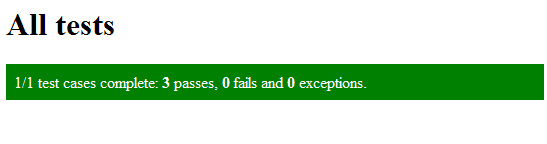
\includegraphics[width=0.7\textwidth]{example1}
    \caption{Green Bar!}
    \label{fig:diagram}
\end{figure}

\section{Playtest second!}
Now that we have a passing test, we want to display some results as web pages.
The following examples utilize the Prado framework to display and manipulate
the database through SQLMap. Since SQLMap framework and Prado framework solve
different problems, they are both fairly independent, they can be used
together or separately.

\subsection{SQLMap and Prado}
To setup Prado, we need to create the follow files and directory structure
under our \tt{example/WebView} directory.
\begin{verbatim}
assets/                         % application public assets

protected/pages/Home.page       % default page
protected/pages/Home.php        % default page class
protected/runtime/              % run time data

protected/application.xml       % application configuration

index.php                       % application entry point
\end{verbatim}

The \tt{application.xml} and \tt{assets} directory are not necessary but we
will make use of them later. The \tt{application.xml} is used to define some
directory aliases and override the data source definitions in the
\tt{sqlmap.config}. This is because SQLite database files are defined
relatively, otherwise we don't need to override the data source definitions.
The example \tt{application.xml} is show in Example~\ref{example:2.0}.

\begin{example}\label{example:2.0}
Prado application.xml, defines path aliases and override SQLite database
location.
\begin{verbatim}
<?xml version="1.0" encoding="utf-8"?>
<application id="SQLMap Example" Mode="Debug">
  <paths>
    <alias id="Example" path="../../" />
    <using namespace="System.DataAccess.*" />
  </paths>
  <modules>
    <module id="SQLMap" class="TSQLMap"
            configFile="Example.sqlmap">
        <!-- override sqlmap.config's database provider -->
        <provider class="TAdodbProvider">
            <datasource driver="sqlite" host="../Data/test.db" />
        </provider>
    </module>
  </modules>
</application>
\end{verbatim}
\end{example}

The entry point to a Prado application in this example is \tt{index.php}.
Example~\ref{example:2.1} shows the basic \tt{index.php} content.
\begin{example}\label{example:2.1}
Prado application entry point, \tt{index.php}.
\begin{verbatim}
<?php
error_reporting(E_ALL);
require_once('/path/to/prado/framework/prado.php');
$application=new TApplication;
$application->run();
?>
\end{verbatim}
\end{example}

Now we are ready to setup a page to display our list of people.
Example~\ref{example:7} shows the Prado code for our display page. The key
piece is the TDataGrid.

\begin{example}\label{example:7}
Prado page for our Person list, \tt{Home.page}.
\begin{verbatim}
<!doctype html public "-//W3C//DTD XHTML 1.0 Strict//EN"
    "http://www.w3.org/TR/xhtml1/DTD/xhtml1-strict.dtd">
<html xmlns="http://www.w3.org/1999/xhtml" lang="en">
<head>
    <title>Person</title>
</head>
<body>
<com:TForm>
    <h1>Person List</h1>
    <com:TDataGrid id="personList">
        <com:TBoundColumn DataField="BirthDate"
                HeaderText="Birth Date"/>
    </com:TDataGrid>
</com:TForm>
</body>
</html>
\end{verbatim}
\end{example}

Of course, we still need to populate that TDataGrid. Example~\ref{example:8}
shows the PHP code for \tt{Home.php}. The operative method is \tt{loadData()}.
The rest is supporting code.

\begin{example}\label{example:8}
\tt{Home.php} class for our Person list page
\begin{verbatim}
<?php
Prado::using('Example.Models.Person');
class Home extends TPage
{
    private function loadData()
    {
        $sqlmap = $this->Application->getModule('SQLMap')->getClient();
        $this->personList->DataSource = $sqlmap->queryForList('SelectAll');
        $this->personList->dataBind();
    }

    public function onLoad($param)
    {
        if(!$this->IsPostBack)
            $this->loadData();
    }
}
?>
\end{verbatim}
\end{example}

If we run this now, we'll get a list like the one shown in
Figure~\ref{figure:2}.
\begin{figure}[!h]
    \centering
        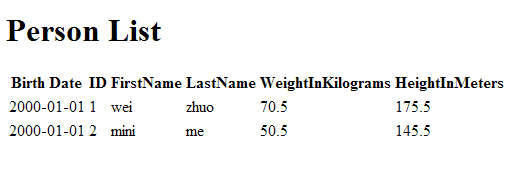
\includegraphics[width=0.75\textwidth]{grid1}
    \caption{A quick-and-dirty Person List}
    \label{figure:2}
\end{figure}

\section{Test, test, again ...}
Of course, tweaking the Person List display is not going to be the end of it.
Clients always want more, and now ours wants to edit, add, or delete records.
Let's write some tests for these new tasks, as shown in
Example~\ref{example:9}.

\begin{example}\label{example:9}
New stories, new tests
\begin{verbatim}
    function testPersonUpdate()
    {
        $expect = "wei";
        $edited = "Nah";

        //get it;
        $person = TMapper::instance()->queryForObject("Select", 1);

        //test it
        $this->assertNotNull($person);
        $this->assertEqual($expect, $person->FirstName);

        //change it
        $person->FirstName = $edited;
        TMapper::instance()->update("Update", $person);

        //get it again
        $person = TMapper::instance()->queryForObject("Select", 1);

        //test it
        $this->assertEqual($edited, $person->FirstName);

        //change it back
        $person->FirstName = $expect;
        TMapper::instance()->update("Update", $person);
    }

    function testPersonDelete()
    {
        //insert it
        $person = new Person;
        $person->ID = -1;
        TMapper::instance()->insert("Insert", $person);

        //delte it
        $count = TMapper::instance()->delete("Delete", -1);
        $this->assertEqual(1, $count);
    }
\end{verbatim}
\end{example}

Not the best tests ever written, but for now, they will do :)

To make the new tests work, we'll need some new mapping statements.
Example~\ref{example:10} shows the complete mapper document that we've called
\tt{personHelper.xml}.

\begin{example}
The new and improved mapper document
\begin{verbatim}
<?xml version="1.0" encoding="utf-8" ?>

<sqlMap Name="PersonHelper">
  <select id="Select" parameterClass="int" resultClass="Person">
   select
    PER_ID as ID,
    PER_FIRST_NAME as FirstName,
    PER_LAST_NAME as LastName,
    PER_BIRTH_DATE as BirthDate,
    PER_WEIGHT_KG as WeightInKilograms,
    PER_HEIGHT_M as HeightInMeters
    from PERSON
    WHERE
      PER_ID = #value#
  </select>

  <insert id="Insert" parameterClass="Person">
   insert into PERSON
    (PER_ID, PER_FIRST_NAME, PER_LAST_NAME,
    PER_BIRTH_DATE, PER_WEIGHT_KG, PER_HEIGHT_M)
   values
    (#ID#, #FirstName#, #LastName#,
    #BirthDate#, #WeightInKilograms#, #HeightInMeters#)
  </insert>

  <update id="Update" parameterClass="Person">
   update PERSON set
    PER_FIRST_NAME = #FirstName#,
    PER_LAST_NAME = #LastName#,
    PER_BIRTH_DATE = #BirthDate#,
    PER_WEIGHT_KG = #WeightInKilograms#,
    PER_HEIGHT_M = #HeightInMeters#
   where PER_ID = #ID#
  </update>

  <delete id="Delete" parameterClass="int">
   delete from PERSON
   where PER_ID = #value#
  </delete>
</sqlMap>
\end{verbatim}
\end{example}
Well, waddya know, if run our tests now, we are favored with a green bar!. It
all works!

\begin{mybox}{Note:}
Though, of course, things usually do not work perfectly the first time! We
have to fix this and that, and try, try, again. But SimpleTest makes trying
again quick and easy. You can changes to the XML mapping documents and rerun
the tests! No muss, no fuss.
\end{mybox}

Turning back to our Prado page, we can revamp the TDataGrid to allow in-place
editing and deleting. To add records, we provide a button after the grid that
inserts a blank person for client to edit. The page code is shown as
Example~\ref{example:11}.
\begin{example}\label{example:11}
Prado page code for our enhanced TDataGrid
\begin{verbatim}
    <com:TDataGrid id="personList"
            DataKeyField="ID"
            AutoGenerateColumns="False"
            OnEditCommand="editPerson"
            OnUpdateCommand="updatePerson"
            OnCancelCommand="refreshList"
            OnDeleteCommand="deletePerson">
        <com:TBoundColumn DataField="FirstName" HeaderText="First Name" />
        <com:TBoundColumn DataField="LastName" HeaderText="Last Name" />
        <com:TBoundColumn DataField="HeightInMeters" HeaderText="Height" />
        <com:TBoundColumn DataField="WeightInKilograms" HeaderText="Weight" />
        <com:TEditCommandColumn
                HeaderText="Edit"
                UpdateText="Save" />
        <com:TButtonColumn
                HeaderText="Delete"
                Text="Delete"
                CommandName="delete"/>
    </com:TDataGrid>
    <com:TButton Text="Add" OnClick="addNewPerson" />
\end{verbatim}
\end{example}

Example~\ref{example:12} shows the corresponding methods from page PHP class.

\begin{example}\label{example:12}
The page class code for our enhanced TDataGrid
\begin{verbatim}
    private function sqlmap()
    {
        return $this->Application->getModule('SQLMap')->getClient();
    }

    private function loadData()
    {
        $this->personList->DataSource =
                $this->sqlmap()->queryForList('SelectAll');
        $this->personList->dataBind();
    }

    public function onLoad($param)
    {
        if(!$this->IsPostBack)
            $this->loadData();
    }

    protected function editPerson($sender,$param)
    {
        $this->personList->EditItemIndex=$param->Item->ItemIndex;
        $this->loadData();
    }

    protected function deletePerson($sender, $param)
    {
        $id = $this->getKey($sender, $param);
        $this->sqlmap()->update("Delete", $id);
        $this->loadData();
    }

    protected function updatePerson($sender, $param)
    {
        $person = new Person();
        $person->FirstName = $this->getText($param, 0);
        $person->LastName = $this->getText($param, 1);
        $person->HeightInMeters = $this->getText($param, 2);
        $person->WeightInKilograms = $this->getText($param, 3);
        $person->ID = $this->getKey($sender, $param);
        $this->sqlmap()->update("Update", $person);
        $this->refreshList($sender, $param);
    }

    protected function addNewPerson($sender, $param)
    {
        $person = new Person;
        $person->FirstName = "-- New Person --";
        $this->sqlmap()->insert("Insert", $person);
        $this->loadData();;
    }

    protected function refreshList($sender, $param)
    {
        $this->personList->EditItemIndex=-1;
        $this->loadData();
    }

    private function getText($param, $index)
    {
        $item = $param->Item;
        return $item->Cells[$index]->Controls[0]->Text;
    }

    private function getKey($sender, $param)
    {
        return $sender->DataKeys[$param->Item->DataSourceIndex];
    }
\end{verbatim}
\end{example}

OK, we are CRUD complete! There's more we could do here. In particular, we
should add validation methods to prevent client from entering alphabetic
characters where only numbers can live. But, that's a different Prado
tutorial, and this is an SQLMap DataMapper tutorial.

\begin{figure}[!h]
    \centering
        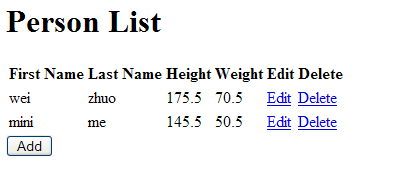
\includegraphics[width=0.75\textwidth]{grid2}
    \caption{Person List CRUD}
    \label{figure:2}
\end{figure}



\end{document}
